\documentclass[border=10pt]{standalone}
\usepackage{amsmath}
\usepackage{tikz}
\usepackage{graphicx}
\usetikzlibrary{positioning, shapes.geometric, arrows.meta, calc, shadows.blur, decorations.pathreplacing, fit, backgrounds, shapes.multipart}

% Define beautiful pastel colors
\definecolor{supportcolor}{RGB}{193, 225, 193}  % Mint green
\definecolor{querycolor}{RGB}{255, 229, 180}    % Peach
\definecolor{encodercolor}{RGB}{255, 204, 204}  % Light pink
\definecolor{lstmcolor}{RGB}{204, 229, 255}     % Light blue
\definecolor{attncolor}{RGB}{255, 218, 185}     % Moccasin
\definecolor{metriccolor}{RGB}{230, 230, 250}   % Lavender
\definecolor{outputcolor}{RGB}{255, 245, 157}   % Light yellow
\definecolor{bordercolor}{RGB}{100, 100, 100}   % Dark gray
\definecolor{tensor3dfront}{RGB}{100, 150, 220} % 3D front face
\definecolor{tensor3dtop}{RGB}{140, 180, 240}   % 3D top face
\definecolor{tensor3dside}{RGB}{70, 120, 190}   % 3D side face

% Commands for drawing 3D tensor blocks
% Cubic block for 2D tensors (batches of features)
\newcommand{\drawcube}[4]{
    % #1 = x position, #2 = y position
    % #3 = size (width/height/depth are similar for cubic)
    % #4 = fill color
    \begin{scope}[shift={(#1,#2)}]
        % Front face (square)
        \fill[#4!80, draw=black, thick] (0,0) rectangle (#3,#3);
        % Top face
        \fill[#4!95, draw=black, thick] (0,#3) -- (#3*0.4,#3+#3*0.4) -- (#3+#3*0.4,#3+#3*0.4) -- (#3,#3) -- cycle;
        % Side face
        \fill[#4!60, draw=black, thick] (#3,0) -- (#3+#3*0.4,#3*0.4) -- (#3+#3*0.4,#3+#3*0.4) -- (#3,#3) -- cycle;
    \end{scope}
}

% Elongated bar for 1D tensors - VERTICAL orientation
\newcommand{\drawbar}[5]{
    % #1 = x position, #2 = y position
    % #3 = length (elongated dimension)
    % #4 = thickness (cross-section size)
    % #5 = fill color
    \begin{scope}[shift={(#1,#2)}]
        % Front face (elongated rectangle)
        \fill[#5!80, draw=black, thick] (0,0) rectangle (#4,#3);
        % Top face
        \fill[#5!95, draw=black, thick] (0,#3) -- (#4*0.5,#3+#4*0.5) -- (#4+#4*0.5,#3+#4*0.5) -- (#4,#3) -- cycle;
        % Side face
        \fill[#5!60, draw=black, thick] (#4,0) -- (#4+#4*0.5,#4*0.5) -- (#4+#4*0.5,#3+#4*0.5) -- (#4,#3) -- cycle;
    \end{scope}
}

% Elongated bar for 1D tensors - HORIZONTAL orientation
\newcommand{\drawhbar}[5]{
    % #1 = x position, #2 = y position
    % #3 = length (elongated dimension - horizontal)
    % #4 = thickness (cross-section size)
    % #5 = fill color
    \begin{scope}[shift={(#1,#2)}]
        % Front face (elongated rectangle - horizontal)
        \fill[#5!80, draw=black, thick] (0,0) rectangle (#3,#4);
        % Top face
        \fill[#5!95, draw=black, thick] (0,#4) -- (#4*0.5,#4+#4*0.5) -- (#3+#4*0.5,#4+#4*0.5) -- (#3,#4) -- cycle;
        % Side face
        \fill[#5!60, draw=black, thick] (#3,0) -- (#3+#4*0.5,#4*0.5) -- (#3+#4*0.5,#4+#4*0.5) -- (#3,#4) -- cycle;
    \end{scope}
}

\begin{document}
\begin{tikzpicture}[
    mainbox/.style={
        rectangle, rounded corners=8pt, draw=bordercolor, thick,
        minimum height=1.2cm, align=center, font=\small\sffamily,
        blur shadow={shadow blur steps=5, shadow xshift=2pt, shadow yshift=-2pt}
    },
    modulebox/.style={
        rectangle, rounded corners=8pt, draw=bordercolor, thick,
        minimum width=2.86cm, minimum height=1.3cm, align=center, font=\large\sffamily,
        blur shadow={shadow blur steps=5, shadow xshift=2pt, shadow yshift=-2pt}
    },
    smallbox/.style={
        rectangle, rounded corners=5pt, draw=bordercolor, thick,
        minimum width=2.34cm, minimum height=1.04cm, align=center, font=\normalsize\sffamily
    },
    inputbox/.style={
        rectangle, rounded corners=8pt, draw=bordercolor, very thick,
        minimum width=3.9cm, minimum height=4.16cm, align=center, font=\Large\sffamily,
        blur shadow={shadow blur steps=5, shadow xshift=2.6pt, shadow yshift=-2.6pt}
    },
    arrow/.style={-{Stealth[scale=1.2]}, thick},
    bigarrow/.style={-{Stealth[scale=1.5]}, very thick},
    formulabox/.style={
        rectangle, rounded corners=5pt, fill=yellow!20, draw=orange!60, thick,
        font=\large, align=center, minimum height=1.04cm
    },
    container/.style={
        rectangle, rounded corners=10pt, draw=bordercolor, dashed, very thick,
        inner sep=12pt
    }
]

%%%%%%%%%%%%%%%%%%%%%%%%%%%%%%%%%%%%%%%%%%%%%%%%%%%%%%%%%%%%%%%%%
% TITLE - Dời lên cao hơn để không đè lên components
%%%%%%%%%%%%%%%%%%%%%%%%%%%%%%%%%%%%%%%%%%%%%%%%%%%%%%%%%%%%%%%%%
\node[font=\Huge\bfseries, color=blue!70] at (14, 9.5) {2-Way Few-Shot Classification Architecture};

%%%%%%%%%%%%%%%%%%%%%%%%%%%%%%%%%%%%%%%%%%%%%%%%%%%%%%%%%%%%%%%%%
% SUPPORT BRANCH (TOP)
%%%%%%%%%%%%%%%%%%%%%%%%%%%%%%%%%%%%%%%%%%%%%%%%%%%%%%%%%%%%%%%%%

% Support Set Input với ảnh placeholder
\node[inputbox, fill=supportcolor] (support) at (0, 5) {
    \textbf{Support Set}\\[0.2cm]
    % Placeholder cho 2 class images
    \begin{tabular}{cc}
        % Option 1: Nếu bạn có file ảnh thật, uncomment dòng dưới
        \includegraphics[width=1.56cm, height=1.56cm]{C002.png} &
        \includegraphics[width=1.56cm, height=1.56cm]{S002.png} \\
        
        % Option 2: Placeholder boxes (comment out if using real images)
        % \tikz{\draw[fill=red!30] (0,0) rectangle (1.2,1.2);} &
        % \tikz{\draw[fill=blue!30] (0,0) rectangle (1.2,1.2);} \\
        
        \Large Corona & \Large Surface
    \end{tabular}\\[0.15cm]
    \tiny{$\mathcal{S} = \{(x_i, y_i)\}_{i=1}^{2K}$}\\
    \tiny{(2-way, K-shot)}
};

% Support Encoder - CNN
\node[modulebox, fill=encodercolor, right=2cm of support] (s_conv) {CNN\\Encoder\\[0.1cm]ResNet};

% Support Encoder - BiLSTM with 3D tensor visualization
% Input 3D tensor before BiLSTM
\node[right=1.5cm of s_conv] (s_bilstm_in) {
    \begin{tikzpicture}[scale=0.6]
        \drawcube{0}{0}{2.5}{encodercolor}
        \node[font=\tiny, below] at (1.25, -0.3) {$(2K, d)$};
    \end{tikzpicture}
};

% BiLSTM module
\node[modulebox, fill=lstmcolor, right=0.8cm of s_bilstm_in] (s_bilstm) {Bidirectional\\LSTM\\[0.1cm]Context};

% Output 3D tensor after BiLSTM
\node[right=0.8cm of s_bilstm] (s_bilstm_out) {
    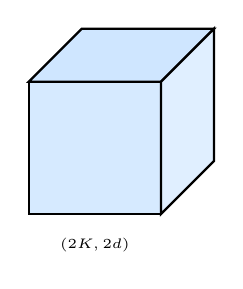
\begin{tikzpicture}[scale=0.6]
        \drawcube{0}{0}{2.8}{lstmcolor}
        \node[font=\tiny, below] at (1.4, -0.3) {$(2K, 2d)$};
    \end{tikzpicture}
};

% Support Encoder - Context
\node[modulebox, fill=attncolor, right=1.5cm of s_bilstm_out] (s_context) {Context\\Embedding\\[0.1cm]Aggregate};

% Support Features Output - IDENTICAL to BiLSTM input (2K,d), only different color
\node[smallbox, fill=supportcolor!50, right=1.5cm of s_context, minimum height=3cm] (s_feat) {
    $g(x_i)$\\[0.1cm]
    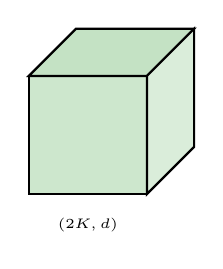
\begin{tikzpicture}[scale=0.6]
        \drawcube{0}{0}{2.5}{supportcolor}
        \node[font=\tiny, below] at (1.25, -0.3) {$(2K, d)$};
    \end{tikzpicture}\\[-0.1cm]
    Support Features
};

% Support encoder container
\node[container, fit={(s_conv) (s_bilstm_in) (s_bilstm) (s_bilstm_out) (s_context)}, label=above:\textbf{Support Encoder $g(\cdot)$}] (support_enc) {};

% Arrows in support branch
\draw[bigarrow] (support.east) -- (s_conv.west);
\draw[arrow] (s_conv.east) -- (s_bilstm_in.west);
\draw[arrow] (s_bilstm_in.east) -- (s_bilstm.west);
\draw[arrow] (s_bilstm.east) -- (s_bilstm_out.west);
\draw[arrow] (s_bilstm_out.east) -- (s_context.west);
\draw[arrow] (s_context.east) -- (s_feat.west);

%%%%%%%%%%%%%%%%%%%%%%%%%%%%%%%%%%%%%%%%%%%%%%%%%%%%%%%%%%%%%%%%%
% QUERY BRANCH (BOTTOM)
%%%%%%%%%%%%%%%%%%%%%%%%%%%%%%%%%%%%%%%%%%%%%%%%%%%%%%%%%%%%%%%%%

% Query Input với ảnh placeholder
\node[inputbox, fill=querycolor] (query) at (0, 0) {
    \textbf{Query Image}\\[0.2cm]
    % Option 1: Nếu bạn có file ảnh thật, uncomment dòng dưới
    \includegraphics[width=2.08cm, height=2.08cm]{C004.png}\\[0.15cm]
    
    % Option 2: Placeholder box (comment out if using real image)
    % \tikz{\draw[fill=orange!30] (0,0) rectangle (1.6,1.6);}\\[0.15cm]
    
    \tiny{$\hat{x}$ (unknown)}
};

% Query Encoder - CNN (aligned with support CNN)
\node[modulebox, fill=encodercolor] (q_conv) at (s_conv |- query) {CNN\\Encoder\\[0.1cm]ResNet};;

% Query Encoder - Attention LSTM with 3D tensor visualization
% Input 3D tensor before Attention LSTM - HORIZONTAL BAR (larger)
\node[right=1.5cm of q_conv] (q_attn_in) {
    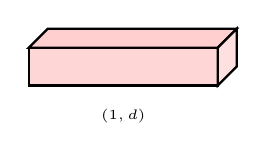
\begin{tikzpicture}[scale=0.6]
        \drawhbar{0}{0}{4.0}{0.8}{encodercolor}
        \node[font=\tiny, below] at (2.0, -0.3) {$(1, d)$};
    \end{tikzpicture}
};

% Attention LSTM module
\node[modulebox, fill=attncolor, right=0.8cm of q_attn_in] (q_attn) {Attention\\LSTM\\[0.1cm]Read Support};

% Output 3D tensor after Attention LSTM - HORIZONTAL BAR (larger)
\node[right=0.8cm of q_attn] (q_attn_out) {
    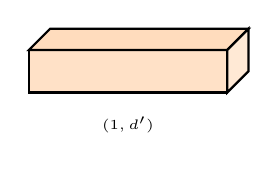
\begin{tikzpicture}[scale=0.6]
        \drawhbar{0}{0}{4.2}{0.9}{attncolor}
        \node[font=\tiny, below] at (2.1, -0.3) {$(1, d')$};
    \end{tikzpicture}
};

% Query Encoder - Context
\node[modulebox, fill=lstmcolor, right=1.5cm of q_attn_out] (q_context) {Query\\Context\\[0.1cm]Embed};

% Query Features Output - IDENTICAL to Attn LSTM input (1,d), only different color
\node[smallbox, fill=querycolor!50, right=1.5cm of q_context, minimum height=3cm] (q_feat) {
    $f(\hat{x})$\\[0.1cm]
    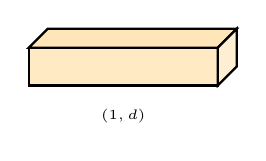
\begin{tikzpicture}[scale=0.6]
        \drawhbar{0}{0}{4.0}{0.8}{querycolor}
        \node[font=\tiny, below] at (2.0, -0.3) {$(1, d)$};
    \end{tikzpicture}\\[-0.1cm]
    Query Feature
};

% Query encoder container
\node[container, fit={(q_conv) (q_attn_in) (q_attn) (q_attn_out) (q_context)}, label=above:\textbf{Query Encoder $f(\cdot)$}] (query_enc) {};

% Arrows in query branch
\draw[bigarrow] (query.east) -- (q_conv.west);
\draw[arrow] (q_conv.east) -- (q_attn_in.west);
\draw[arrow] (q_attn_in.east) -- (q_attn.west);
\draw[arrow] (q_attn.east) -- (q_attn_out.west);
\draw[arrow] (q_attn_out.east) -- (q_context.west);
\draw[arrow] (q_context.east) -- (q_feat.west);

%%%%%%%%%%%%%%%%%%%%%%%%%%%%%%%%%%%%%%%%%%%%%%%%%%%%%%%%%%%%%%%%%
% CROSS-CONNECTIONS - Routing để không đi qua components
%%%%%%%%%%%%%%%%%%%%%%%%%%%%%%%%%%%%%%%%%%%%%%%%%%%%%%%%%%%%%%%%%

% Shared weights between CNNs - đi thẳng giữa 2 CNN
\draw[bigarrow, dashed, color=purple, line width=2pt] (s_conv.south) -- 
    node[left, font=\normalsize\bfseries, color=purple, fill=white, inner sep=2pt] {Shared Weights} (q_conv.north);

% Attention: Query reads Support - đường cong mượt
\draw[arrow, dashed, color=red!70, line width=1.5pt] 
    (s_bilstm_out.south) to[out=-90, in=90] 
    node[midway, left, font=\normalsize, color=red!70, fill=white, inner sep=2pt] {Attention Read}
    (q_attn.north);
%%%%%%%%%%%%%%%%%%%%%%%%%%%%%%%%%%%%%%%%%%%%%%%%%%%%%%%%%%%%%%%%%
% MATCHING NETWORK (RIGHT SIDE) - Dời sang phải hơn
%%%%%%%%%%%%%%%%%%%%%%%%%%%%%%%%%%%%%%%%%%%%%%%%%%%%%%%%%%%%%%%%%

% Cosine Similarity - Tăng khoảng cách sang phải
\node[modulebox, fill=white, minimum width=3.64cm, right=3.5cm of s_feat, yshift=-2.5cm] (cosine) {
    Cosine\\Similarity\\[0.1cm]
    \Huge{$c_i = \cos(f(\hat{x}), g(x_i))$}
};

% Softmax Attention
\node[modulebox, fill=white, minimum width=3.64cm, below=1cm of cosine] (softmax) {
    Softmax\\Attention\\[0.1cm]
    \Huge{$a_i = \frac{\exp(c_i)}{\sum_j \exp(c_j)}$}
};

% Formula Box
\node[formulabox, minimum width=4.55cm, right=1.2cm of softmax] (formula) {
    $a(\hat{x}, x_i) = \frac{\exp(c_i)}{\sum_{j=1}^{2K} \exp(c_j)}$
};

% Weighted Voting
\node[modulebox, fill=outputcolor, minimum width=4.16cm, minimum height=1.56cm, below=1.2cm of softmax] (voting) {
    \textbf{Weighted Voting}\\[0.1cm]
    \Huge{$\hat{y} = \sum_{i=1}^{2K} a_i y_i$}
};

% Output Prediction
\node[smallbox, fill=outputcolor!70, minimum width=8.45cm, minimum height=1.56cm, below=1cm of voting] (scores) {
    \textbf{Prediction}\\[0.1cm]
    \Huge{$[0.78, 0.22]$}\\
    \Huge{$[P(\text{Corona}), P(\text{Surface})]$}
};

%%%%%%%%%%%%%%%%%%%%%%%%%%%%%%%%%%%%%%%%%%%%%%%%%%%%%%%%%%%%%%%%%
% MATCHING CONTAINER - Vẽ TRƯỚC trên background layer
%%%%%%%%%%%%%%%%%%%%%%%%%%%%%%%%%%%%%%%%%%%%%%%%%%%%%%%%%%%%%%%%%

% Container bao quanh TOÀN BỘ matching section - sử dụng background layer
\begin{scope}[on background layer]
    \node[container, fit={(cosine) (softmax) (voting) (scores) (formula)}, 
          fill=metriccolor!30, draw=bordercolor, dashed, very thick,
          inner sep=15pt] (matching) {};
\end{scope}

% Label cho container - vẽ riêng để nổi bật
\node[font=\large\bfseries, above=10pt of matching.north, fill=white, inner sep=4pt] 
    {Attention Mechanism \& Classification};

%%%%%%%%%%%%%%%%%%%%%%%%%%%%%%%%%%%%%%%%%%%%%%%%%%%%%%%%%%%%%%%%%
% ARROWS TO MATCHING - Góc 90 độ rõ ràng
%%%%%%%%%%%%%%%%%%%%%%%%%%%%%%%%%%%%%%%%%%%%%%%%%%%%%%%%%%%%%%%%%

% Arrow từ Support Features - góc 90 độ
\draw[arrow] (s_feat.east) -| (cosine.north);

% Arrow từ Query Features - từ trên xuống bên trái cosine
\draw[arrow] (q_feat.north) |- (cosine.west);

% Arrows trong matching network - đường thẳng
\draw[arrow] (cosine) -- (softmax);
\draw[arrow] (softmax) -- (formula);
\draw[arrow] (softmax) -- (voting);
\draw[arrow] (voting) -- (scores);

%%%%%%%%%%%%%%%%%%%%%%%%%%%%%%%%%%%%%%%%%%%%%%%%%%%%%%%%%%%%%%%%%
% LEGEND
%%%%%%%%%%%%%%%%%%%%%%%%%%%%%%%%%%%%%%%%%%%%%%%%%%%%%%%%%%%%%%%%%
\node[font=\normalsize\bfseries, fill=supportcolor, draw, rounded corners, minimum height=0.6cm] at (2, -3.5) {Input Data};
\node[font=\normalsize\bfseries, fill=encodercolor, draw, rounded corners, minimum height=0.6cm] at (5.2, -3.5) {CNN};
\node[font=\normalsize\bfseries, fill=lstmcolor, draw, rounded corners, minimum height=0.6cm] at (7.8, -3.5) {LSTM};
\node[font=\normalsize\bfseries, fill=attncolor, draw, rounded corners, minimum height=0.6cm] at (10.5, -3.5) {Attention};
\node[font=\normalsize\bfseries, fill=metriccolor, draw, rounded corners, minimum height=0.6cm] at (13.5, -3.5) {Metric};
\node[font=\normalsize\bfseries, fill=outputcolor, draw, rounded corners, minimum height=0.6cm] at (17, -3.5) {Output};

\end{tikzpicture}
\end{document}
